\documentclass[letter,10pt]{article}
\usepackage[utf8x]{inputenc}
\usepackage{graphicx}
\usepackage{url}
\usepackage{amsmath}
\usepackage{amsfonts}

%opening
\title{A path-selection problem for a floating sensor network to optimize sensing objectives}
\author{Kevin Weekly}

\begin{document}

\maketitle

\begin{abstract}
This project will focus on identifying and solving a particular, but extensible problem related to coordination and control of motorized floating sensor units. We begin by providing a general framework for the problems the project will focus on. That is, for each viable path through the water network, we assign a given number of sensors to proceed down that path.  The selection is done to maximise a utility function composed of two decoupled sensing objectives-- a long-term salinity measurement objective, and a short-term pH measurement objective.

The intent is that such problems can be solved repeatedly during a deployment as conditions about the environment are discovered, or the user requirements change.  Therefore, the problems should be able to be solved on a modern desktop computer using either CPLEX or corresponding Python libraries (preferred) in the order of minutes or less.  Also, there may also be some benefit in examining the Lagrange multipliers from these problems to furnish the user with information on the way that constraints are affecting the solution. 
\end{abstract}

\section{The Floating Sensor Network}

The floating sensor network is a fleet of 20 motorized sensors, or ``drifters'', used currently to measure the Lagrangian flow-field of their environment.  A graphical depiction of one sensor is shown in Figure \ref{fig:fsn-drifter}. The river delta the sensors are currently used in is depicted by Figure \ref{fig:fsn-delta}.

\begin{figure}[h]
 \centering
 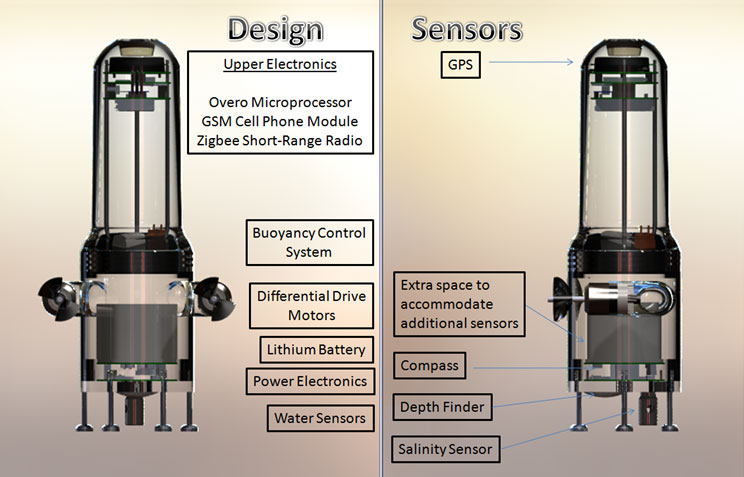
\includegraphics[width=\linewidth ]{figures/fsn.jpg}
 \caption{Floating Sensor Unit\label{fig:fsn-drifter}}
\end{figure}

\begin{figure}[h]
 \centering
 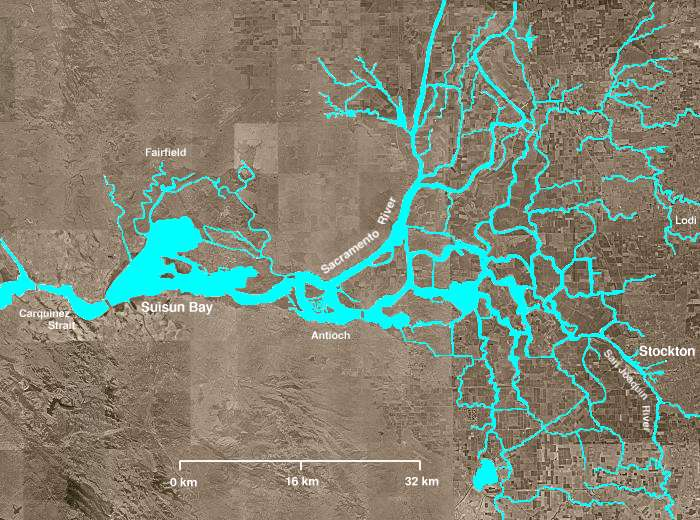
\includegraphics[width=\linewidth ]{figures/Wpdms_usgs_photo_sacramento_delta_2.jpg}
 \caption{Sacramento-San Joaquin River Delta (Source: wikipedia.org)\label{fig:fsn-delta}}
\end{figure}

During a deployment operation, the fleet of 20 are deployed in a region of the San-Joaquin/Sacramento Delta where they float along with the natural current, reporting their GPS position \& salinity measurements over the GSM (cell-phone) network or Zigbee (short-range radio) network.  In the context of deployment, there are effectively two controls at our disposal--
\begin{itemize}
 \item The individual deployment strategy for the fleet from a boat. i.e. when, where, and how many units are deployed from a human-operated motorboat.  This strategy is constrained by the limited speed of boats, their limited mobility in shallow areas (i.e. the drifters can go to some places the boats cannot), and limited capacity (typically can carry 5 units).
 \item The actuation of the drifters themselves.  Using their motors, the units can move themselves in any direction, albiet slowly.  Their control authority is approximately $20 \frac{\mbox{cm}}{\mbox{s}}$ \emph{relative to the water speed} (i.e. in some areas the current is fast enough that the units cannot swim upstream).  They are further constrained by limited battery life, and, were the proposed algorithm to be done in a centralized manner, by lack of communication.
\end{itemize}

\section{Software}

The software/hardware configurations we intend to investigate are listed in Table \ref{tab:configurations}.  It is especially interesting if an algorithm can be made to run with Configuration 3 in reasonable time, since then it could be performed in the field.

\begin{figure}[h]
{%
\newcommand{\mc}[3]{\multicolumn{#1}{#2}{#3}}
\begin{center}
\begin{tabular}{lll}
Configuration & Software & Platform\\
\mc{1}{c}{1} & CPLEX  & PC (Intel i5 2.7GHz)\\
\mc{1}{c}{2} & OpenOpt (glpk)  & PC (Intel i5 2.7GHz)\\
\mc{1}{c}{3} & OpenOpt (glpk) & Overo COM (720MHz)\\
\end{tabular}
\end{center}
}%
\caption{Configurations to be tested.\label{tab:configurations}}
\end{figure}


\section{Dynamic sensor objective optimization}

The floating sensors may serve two sensing purposes-- One is to continuously monitor some chemical in the water, such as salt, to examine long term effects.  Another is to detect short-term disturbances, such as an acid spill which can be detected via a pH sensor.  A graphical depiction is shown by Figure \ref{fig:hetero-sense}.

\begin{figure}[h]
 \centering
 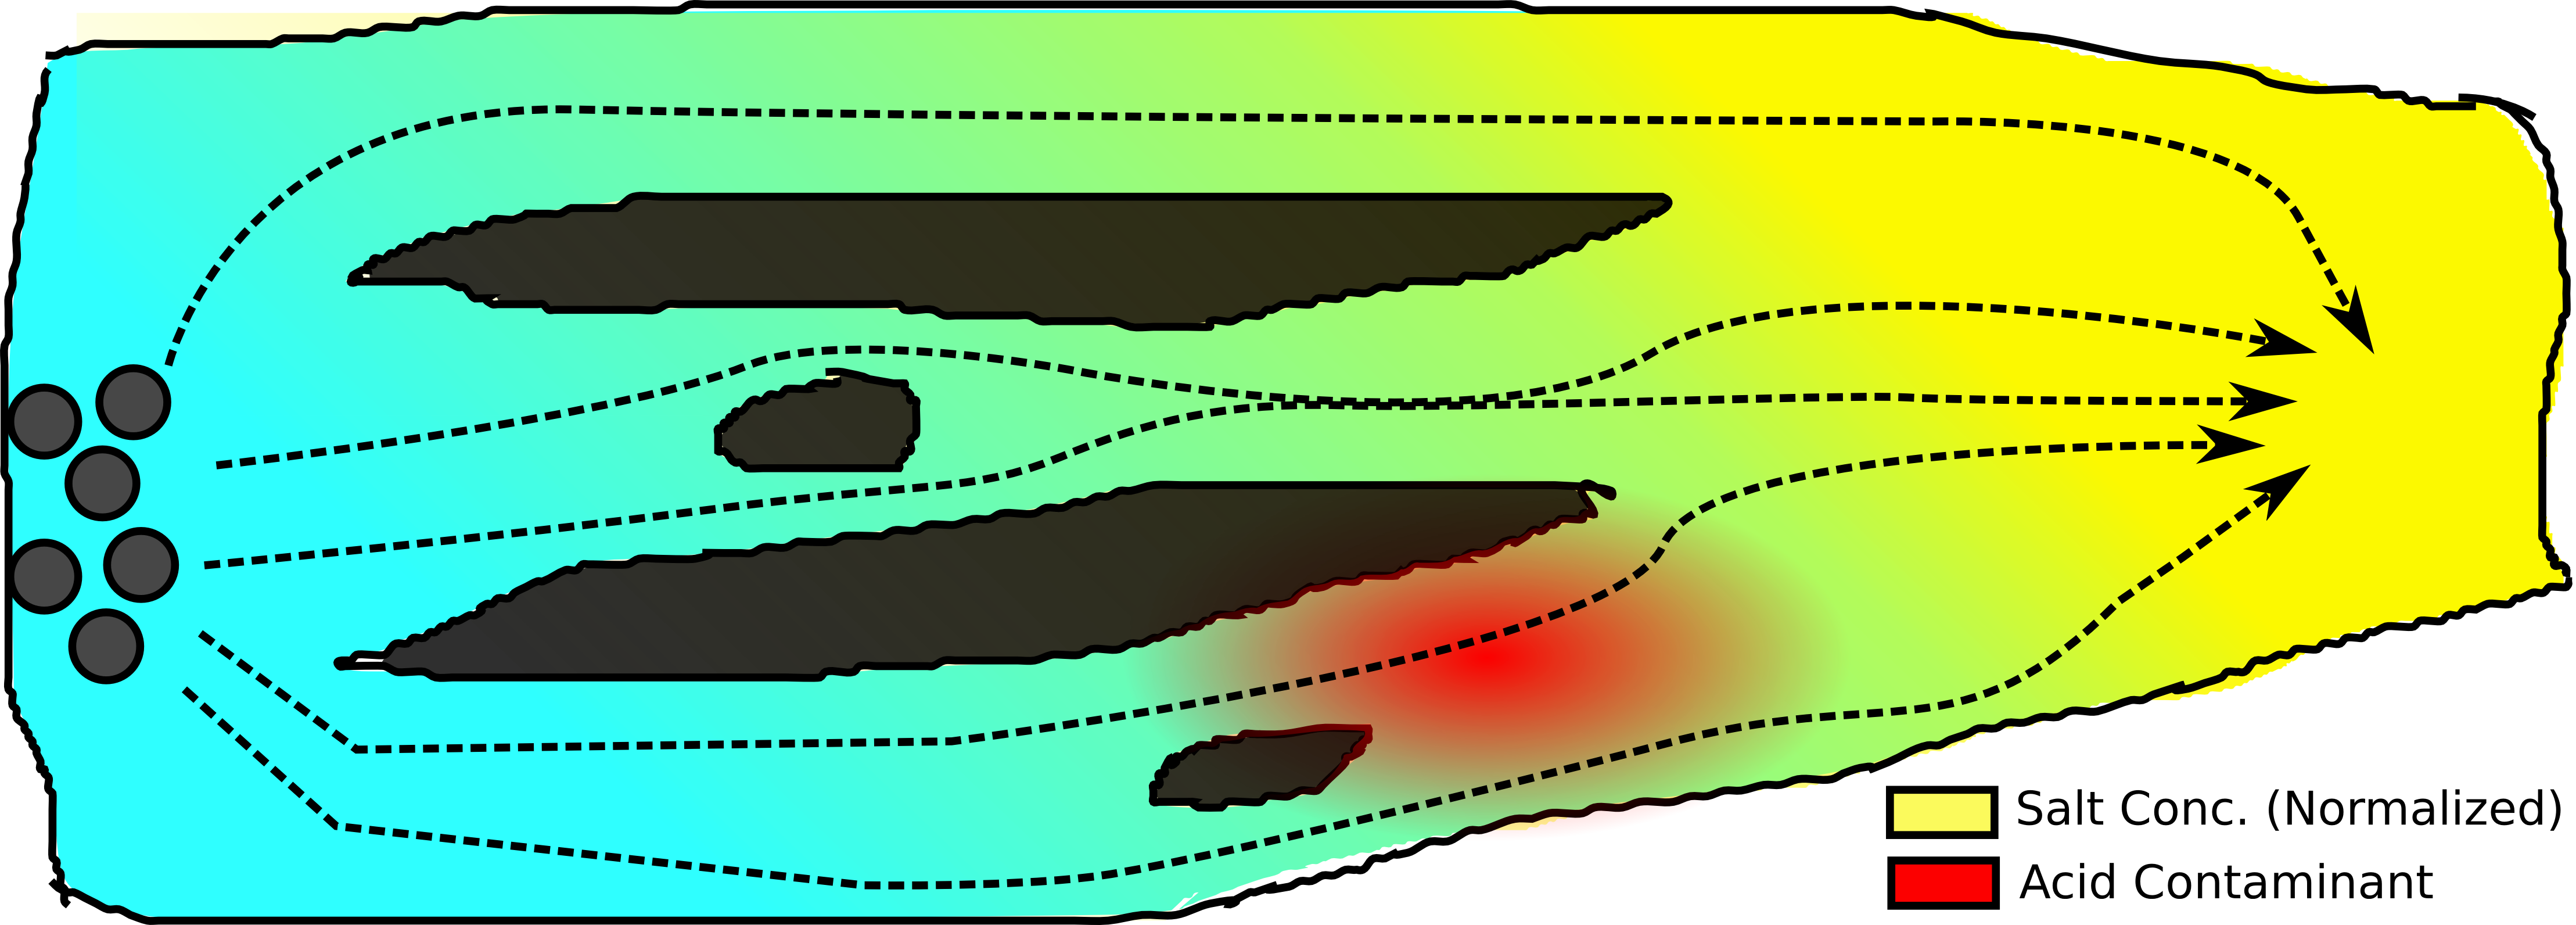
\includegraphics[width=\linewidth ]{figures/combin_river.png}
 \caption{Dual-Purpose Sensing Problem. Dotted lines indicate optimal paths. \label{fig:hetero-sense}}
\end{figure}

The goal is to maintain a certain level of salinity sensing, while also gaining more information about the acid spill with a fixed number of sensors.  The choice variable for this example are the particular paths one could send a sensor through. A particular formulation might be:

\begin{align*}
\max & \; f_s(x) + f_p(x) - c(x)\\
\mbox{s.t.} & \sum_{i=0}^{N} x_i \leq D\\
& c(x_i) \leq B_i 
\end{align*}

Where:
\begin{itemize}
 \item $x_i \in \mathbb{Z}^+ $ are the decision variables, indicating how many units are sent down a path.
 \item $N$ is the number of paths available, or $\vert X\vert$
 \item $f_s$ and $f_p$ are arbitrary utility functions, giving the ``reward'' corresponding to salt and pH measurements, respectively, for taking such paths.
 \item $c(x)$ is a function giving the cost of the assignment, such as the amount of battery power required to drive the sensor to a certain path.
 \item $D$ is the number of sensors available
\end{itemize}

In reality, the location of the chemical spill would be unknown. More likely, a probability distribution might be known based on where runoffs come from farms or where there is a public access road ( which would indicate illegal dumping ), or the location of an industrial plant.  

It could be interesting to explore a choice of $f_s$, $f_p$, and $c$ which do not lead to a greedy optimal solution.  One can imagine that to detect and localize an acid spill, much more than only one sensor would be needed in proximity. Therefore, the marginal utility of $f_p$ could increase as more sensors are added to an area.

For the salinity sensing objective, there would be significant dependence between decision variables in $f_s$.  Consider a small tributary connecting two large branches of the river-- The large branches have a fairly large utility to be sensed. The smaller tributary is fairly insignificant \emph{unless} the two larger branches it connects to are also sensed (i.e. then we can know how much saltwater is crossing between the two ). 

We mostly intend to have $c$ reflect the actuation cost of moving onto a path, a value which is precomputed based on known paths and current location of the units ( this is quite likely another NP-hard problem, but we can probably use a suboptimal solution ).

A hypothesis is that the utility functions described above will lead to an integer program who's solution ``focuses'' on the most important area and assigns a suitable number of sensor units to address the issue.  An example of this type of behavior is shown in \ref{fig:focus}.

\begin{figure}[h]
 \centering
 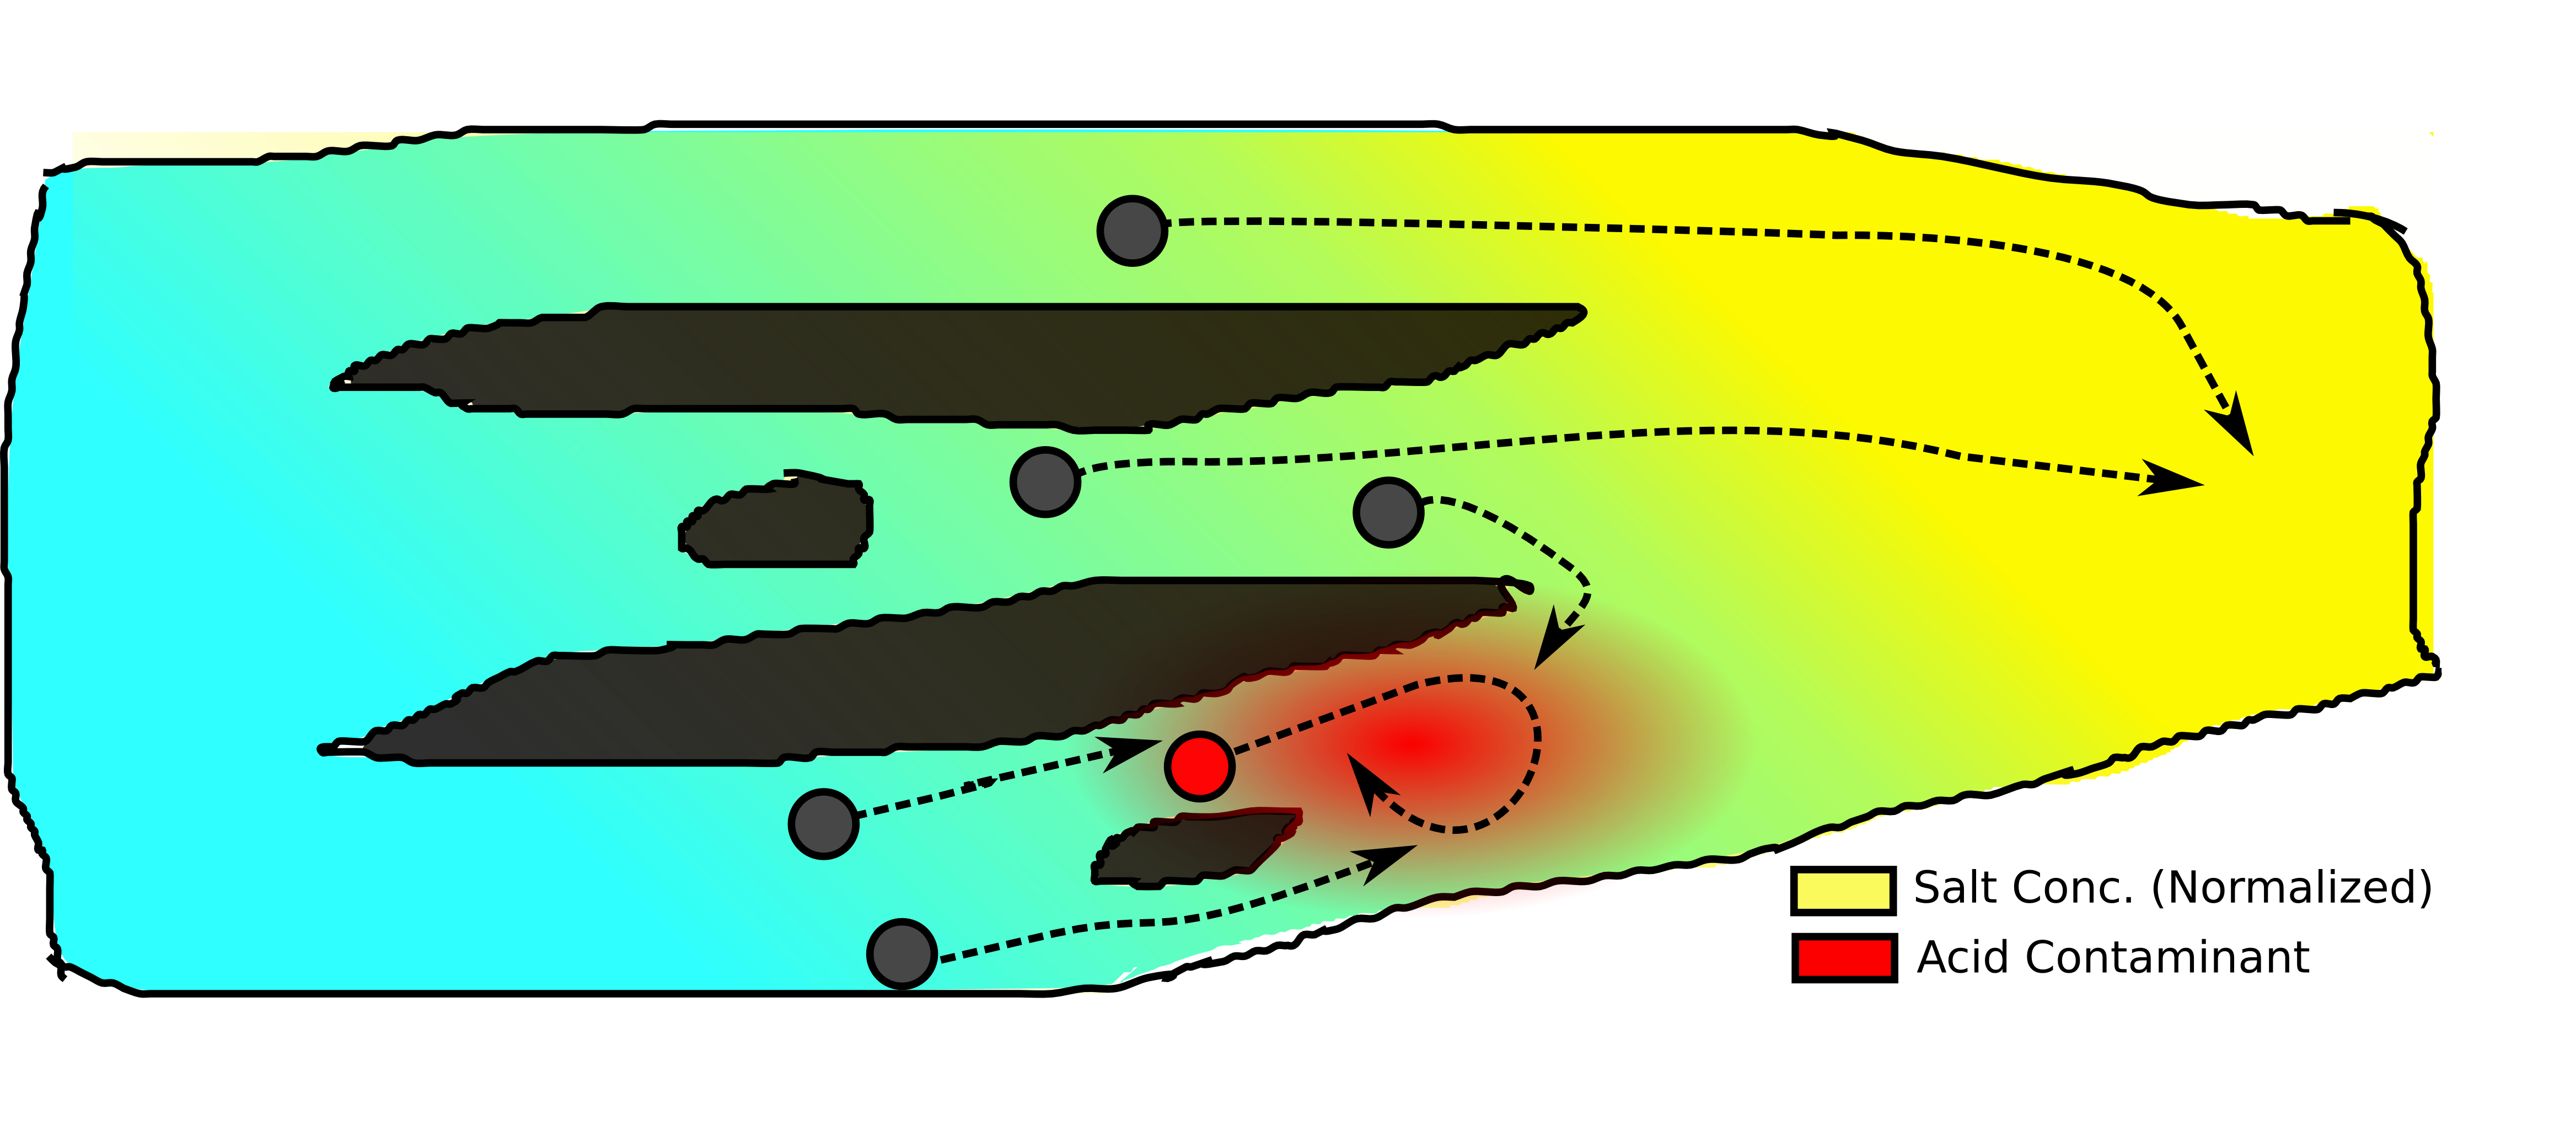
\includegraphics[width=\linewidth ]{figures/combin_river_2.png}
 \caption{Problem is re-solved on-the-fly when a contaminant is detected. Note the actuation costs for some drifters is high enough that they continue on their original mission. \label{fig:focus}}
\end{figure}

Also, if the program is feasible for real-time solving, the utility and cost functions could be updated as areas are sensed or as user objectives change, perhaps causing the fleet to switch its focus to another area of interest, automatically. 


\end{document}
